% -*- coding: utf-8; -*-

\chapter{Introduction}
\begin{itemize}
    \color{red}
    \item What is Reference typing?
    \item What is the main representation (from Pierce)?
    \item What we want to propose studying?
    \item What is our alternative representation?
    \item What are the differences
    \item Why should we formalize an idea?
    \item Which Theorems we want to prove?
    \item Which usabilites can we identify by this formalization?
    \item Is this representation simpler or more complicated to prove?
    \item Is this dissertation meant to be didatic?
\end{itemize}
Type Reference is a technique of representing the types of a program in a store. Some properties of this store can be defined to verify the correctness of a given representation. Formalizing these concepts makes it more understandable, in a way which computer scientists can comunicate their ideas through a standardized set of rules.
Why coq? Coq is a expressive functional programming language used for stating and proving logical assertions and a standard tool for researchers to reason about complex language definitions \cite{Pierce_SF1}

% \begin{figure}
% \centering
% 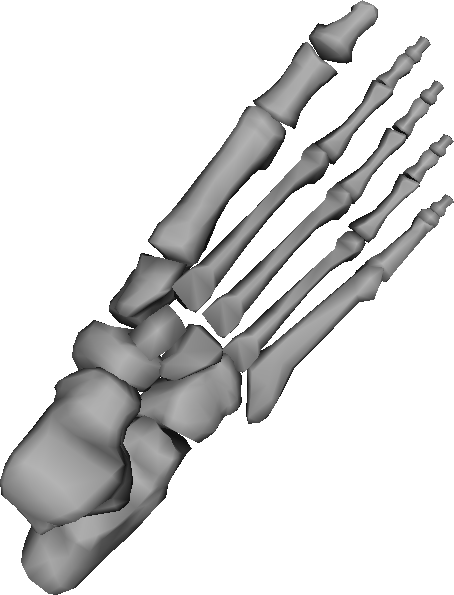
\includegraphics[width=0.45\textwidth]{pictures/image01.png}
% 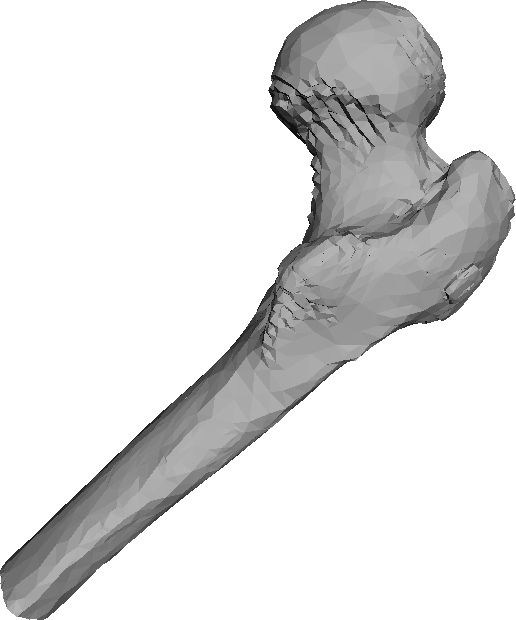
\includegraphics[width=0.45\textwidth]{pictures/image02.png}
% \caption{Meshes generated from medical data. Data obtained from the AIM$@$SHAPE Shape Repository \cite{AIMSHAPE}}
% \label{fig:example}
% \end{figure}


This document is structured as follows. In Chapter~\ref{cha:Previous Work} we present some previous work relevant to our problem. In Chapter~\ref{cha:Proposal} we explain our proposal. In Chapter~\ref{cha:Results} we show our results. Finally, in Chapter~\ref{cha:Conclusion} we present our conclusion and future work.


